\documentclass[sigconf, nonacm]{acmart}

\usepackage{booktabs} % For formal tables
\usepackage{graphicx}
\usepackage[ruled]{algorithm2e} % For algorithms
\renewcommand{\algorithmcfname}{ALGORITHM}
\SetAlFnt{\small}
\SetAlCapFnt{\small}
\SetAlCapNameFnt{\small}
\SetAlCapHSkip{0pt}
\IncMargin{-\parindent}
\setlength\parindent{0pt}


% Document starts

% Title portion
\title{Machine learning models to predict psychometric personality types in order to better understand customer reviews}


\author{Christopher Culley}
\affiliation{%
  \institution{University of Southampton}
  \streetaddress{2 University Rd}
  \city{Southampton}
  \state{Hampshire}
  \postcode{SO17 1BJ}
  \country{UK}}
\email{cc2u18@soton.ac.uk}
\author{Sam Banks}
\affiliation{%
  \institution{University of Southampton}
  \streetaddress{2 University Rd}
  \city{Southampton}
  \state{Hampshire}
  \postcode{SO17 1BJ}
  \country{UK}}
\email{swb1n18@soton.ac.uk}
\author{Fairouz Aldabbagh}
\affiliation{%
  \institution{University of Southampton}
  \streetaddress{2 University Rd}
  \city{Southampton}
  \state{Hampshire}
  \postcode{SO17 1BJ}
  \country{UK}}
\email{fa2n18@soton.ac.uk}
\author{Jak Hall}
\affiliation{%
  \institution{University of Southampton}
  \streetaddress{2 University Rd}
  \city{Southampton}
  \state{Hampshire}
  \postcode{SO17 1BJ}
  \country{UK}}
\email{jh16g18@soton.ac.uk}

\author{Claudia Subia}
\affiliation{%
  \institution{University of Southampton}
  \streetaddress{2 University Rd}
  \city{Southampton}
  \state{Hampshire}
  \postcode{SO17 1BJ}
  \country{UK}}
\email{cms2n17@soton.ac.uk}

\begin{abstract}

In this works we present a predictive model pipeline for determining the personality of business users utilising  comments supporting business review feedback. We use forum comments with attached Myers Briggs personality types in building the models with high accuracy, a mean of 85\% for each of the four letters, and use these models to determine the personality types of Yelp business reviews. We demonstrate the utility of such a pipeline in a web application which allows businesses to understand its reviewer base across the personality types.   

\end{abstract}
\begin{document}

\maketitle

\section{Introduction}

Understanding business reviews can lead to positive structural reforms and highlight areas of progress. Moderate reviews with depth have been shown to be the most beneficial in gaining a deeper understanding of a customer base \cite{mudambi2010research} and extreme reviews can have a detrimental effect on service use \cite{sparks2011impact}. Exploring these two, and other, sets of reviewer personality traits could therefore be a boon to businesses in identifying and responding to customer trends.   \\

Previous studies have explored the personology of consumer behaviour \cite{baumgartner2002toward} and the role of personaility traits in online transactional decision making \cite{bosnjak2007personality} and also personality detection from a corpus of words \cite{mairesse2006automatic} but an emphasis on identifying personality traits in determining business reviewer ratings distributions, to the best of our knowledge, is novel.   \\

In this works we present an analytic application which could help business owners determine which personality types use their service and how favourably, or otherwise, those personality types reviewed the experience. \\


To do so we use a combination of text-processing, machine learning and statistical analysis in determining the personality types of business reviewers and the distribution of ratings across selected businesses which we present in a web application. \\


To understand the personality of users the MBTI (Myers-Briggs Type Indicator) \cite{mccaulley1990myers} can be used to categorise users into personality types. The type indicator is made up of four key factors: Extroversion/Introversion, Sensing/Intuition, Thinking/Feeling and Judging/Perceiving which, together, make up a personality type.\\

We next give a brief summary of each indicator but direct the reader to \cite{mccaulley1990myers} for more details. Extroverted (E) people are energised by social interaction and prefer to share problem solving. Introverted (I) people are drained by social interaction, preferring quiet reflection in their own inner world. They prefer one or two key friendships to group settings. Sensing (S) refers to people who are concerned with practical physical reality and acting in the moment, whilst Intuition (N) refers to people who are less practical, preferring to think things through. A Thinking (T) person processes information based on logic and reason whilst a Feeling (F) person accounts for other peoples feelings, tending to make decisions with their hearts. A Judging (J) person likes to feel in control and lives an ordered, well organised life. A Perceiving (P) person is more flexible and open to new experiences, without planning ahead. A four-letter system is applied to personality types so, for example, an extroverted, sensing, thinking and judging person would be labeled ESTJ. \\

We present the overview pipeline in Figure \ref{method_fig}; we start first with pre-processing the text datasets ready for the machine learning algorithms utilising extensive feature engineering for added predictability, we then build separate models using logistical regression, support vector machines, random forest and a feed-forward neural network applied to a dataset which has user comments linked to their personality type. After comparing the accuracy of each of the models, we use the best four models (one for each binary choice of personality letter) and apply them to a business review dataset linking business reviews with personality types. The final step incorporates these statistical results into a web application. 

\begin{figure}
\includegraphics[width= 0.9\columnwidth]{Methodology_fig.pdf}
\caption{An overview of the method used to create the application, showing each stage in the developmental process in order of occurrence. }
\label{method_fig}
\end{figure}

This paper is structured as follows, we first give details of the datasets used to build the predictive model and then applied on to demonstrate the application. Next we describe the pre-processing steps applied to the raw data followed by the machine learning pipeline. After this, the results section gives the predictive modeling which is followed by the application overview. We close with a discussion and conclusion. 



\section{Data}

We use the Yelp dataset \cite{challenge2013yelp} as data for which we aim to understand the distribution of personality of reviewers. This dataset has been used to build predictive models of business ratings through user text alone \cite{fan2014predicting} and extracting customer subtopics \cite{huang2014improving} owing to is large size and data integrity.  \\

This data supplies over 5 million reviews of all types of businesses for eleven cities across four countries. For our purposes, and for computational limitations, we focus on Las Vegas (USA) but note to the reader that scaling the prototype application to cover the entire dataset is possible with hardware expansion. \\

In order to categorise the reviewers into their personality types we first build a predictive model using and Mbti comments dataset \cite{mbti_data} taken from the PersonalityCafe forum. This dataset contains 8600 users each with multiple comments on the forum accompanied by the users self-proclaimed personality type.   

\section{Ethics}

In order to comply with data protection regulations, we note that people do not use ‘handles’ or usernames when leaving comments, instead proper names are used. These names are be removed in order to preserve anonymity, even though only first names are used in most cases. Secondly, although the comments are used to process and classify personality types, no comment is used in the output data, thus preserving total anonymity. This also prevents the possibility of anyone seeing their comment and taking offense at being classified as a personality type which did not reflect their self-image.


\section{Preprocessing}

Biased datasets reduce the generalisability of predictive models and as such need to be corrected. The MBTi, has clear bias with some letter weightings observed for 75\% of the datapoints. Although there are many options to resolve this \cite{huang2007correcting}, we utilise the simplest though re-sampling separate balanced datasets by target. We do this for each of the four targets in the MBTi dataset, creating four distinct train test sets with balanced targets.   \\

In order to ready the data to build the predictive models we first apply a number of pre-processing steps in order to maximise the opportunity for meaningful patterns to be extracted. We begin by combining reviews from the same person in both the datasets into corpus from with which we apply some feature engineering listed in Table \ref{feature_engineering}. We note to the reader, the sentiment analysis features, polarity and subjectivity as well as the word probability information were applied, using the NLTK library \cite{bird2004nltk}, to each users with the listed statistics captured over the individuals aggregated corpus. \\

We next turn the corpus into a bag-of-words where each instance of a word in a corpus corresponds to count in a column. We do this for the 5,000 most common lemmatised words found inside the MBTi dataset ignoring stopwords. We take forward in total 5,017 features to be used inside the machine learning models. \\

At this point we note to the reader the quandary of scaling. Since scaling the data is a requirement for some algorithms, such as the SVM, and leads to faster solution convergence for neural networks \cite{lecun2012efficient} we need to apply scaling to the MBTi. In situations when it is expected that train-test splits are of the same distributions one would normally  minus the train mean and divide by the train standard deviation for all data-points in both the train and test set which, in the MBTi case, presents no problem. \\ 

The problem arises when we want to next apply the model learned from the MBTi to the Yelp data. Which, may follow a different distribution, this is particularly pronounced when there is more data per corpus (and thus a higher average word count). To overcome this, we normalise the Yelp data using its own mean and standard deviation which we found empirically gave a distribution of targets closer to which is expected in the general population but note this highlights a limitation in our generalisation approach -- applying machine learning models from one source to another. 

\begin{table}
\begin{tabular}{ | c | }
\hline
Features Extracted  \\
\hline 
Average word length  \\
Max polarity \\
Min polarity \\
Average polarity \\
Max subjectivity \\
Min subjectivity \\
Average subjectivity \\
Percentage of words misspelled \\
Average misspelled word length \\
Max word probability \\
Average word probability \\
Standard deviation of word probabilities \\
Percentage of words that are emoticons  \\
Percentage of letters that are punctuation \\
Percentage of words that are uppercase \\ (excluding single letters) \\
Percentage of letters that are numerical \\
Percentage of words that are stop words \\
\hline 
\end{tabular}

\caption{The features extracted from the corpus of words defined by each user in both the MBTi and the Yelp datasets}
\label{feature_engineering}
\end{table} 

\section{Machine Learning}

To build the predictive models which we will later apply to the Yelp dataset, we explore four machine learning models which we apply to each of the binary decisions available that construct together to create the four letter personality type. The machine learning algorithms we explore are as follows: logistical regression -- selected for its simplicity as a benchmark, support vector machines -- shown to work well with prediction models for text applications, random forests -- an ensemble method popular also for text prediction problems and a feed-forward neural network -- for its ability to construct highly complex latent variables. \\

For each of the predictive model training we use a pipeline of 5 fold cross validation to tune any hyper-parameters and calculate the accuracy scores using a held out test set. 

We next discuss briefly each of the algorithms. \\

\subsection{Logistic Regression}

Logistic Regression is a regression algorithm commonly used for classification. It uses a logistic function to calculates the probability of the data belonging to a class or not and outputs it as a binary value between 0/No and 1/Yes \cite{hosmer2000applied}. Logistic Regression allows working with highly interdependent features and it can support millions of features in the model and there is no need to define similarity function. It is faster at classification other standard methods such as k nearest-neighbors. This method has few parameters, but since we use gradient decent as an optimisation procedure we determine before hand the maximum number of iterations. \\


\subsection{SVM}

The support Vector Machine (SVM) is a supervised machine learning algorithm used for both linear or nonlinear classification, regression (SVR variant), and outlier detection\cite{geron2017hands}. An SVM is able to project the data points into some new vector space of potentially infinite dimensions where the data is linearly separable. Importantly, rather than have to project all data points into this space, the algorithm only requires a similarity calculation between data points in this new space making the SVM computationally efficient for even the most complex projections.  \\

The SVM is well suited to complex classification problems with small or medium-sized datasets. SVM models are used in text classification problems due to strong performance when working with high dimensional data such as text \cite{wang2006optimal, vapnik2013nature}.\\

In order to use this model it is important to scale the data because SVM models are very sensitive to feature scales \cite{joachims1998text} which we account for in the pre-processing stage. \\

We use an radial basis function kernel to project the data and tune the error allowance of the Lagrangian multipliers in the cross validation stage. 

\subsection{Random Forest}
Random Forest \cite{breiman2001random} are ensemble classification models based on multiple decision trees, which use entropy to select conditional splits leading to prediction outputs, trained using different combinations of the available data and features with bagged voting outputs.  \\

Random forests benefit from having very few hyper parameters to tune such as the minimum tree height and the minimum samples in a split
which we again find using cross validation. 

\subsection{Feed Forward Neural Network}

A feed forward neural network is an acyclic network of nodes with weighted connections between distinct layers with non-linear activation functions applied to the summed input of a node to give the output which is passed as input to the next layer \cite{lippmann1987introduction}. \\

After grid searching the hyper parameters we opt for the input vectors connected to four hidden layers each with 75 neurons. We follow others in using dropout and maxnorm regularisation \cite{srivastava2014dropout} to reduce over-fitting. We use Relu activation function on the inner layers and a binary cross-entropy on the output with ADAM optimiser \cite{kingma2014adam}. 


\section{Machine Learning Results}

We present the machine learning results in Table \ref{ModelResults} and schematically in Figure \ref{fig_ml_models_results} . We achieve strong accuracy rates across each of the models with high accuracy rate. Taking the strongest performing model for each of the classification problems we score an mean accuracy of 86\%. We note that the strongest performing model was logistical regression in all but one case which, as one of the simplest methods available, demonstrates the importance of feature engineering in building text classification models. \\

In Figure \ref{feature_importance} we give the engineered features ranked by importance for each of the models, measured by contributing coefficient. We note with interest the large variability of ranking of these features depending on the letter being predicted.


\begin{figure}
\begin{tabular}{c}
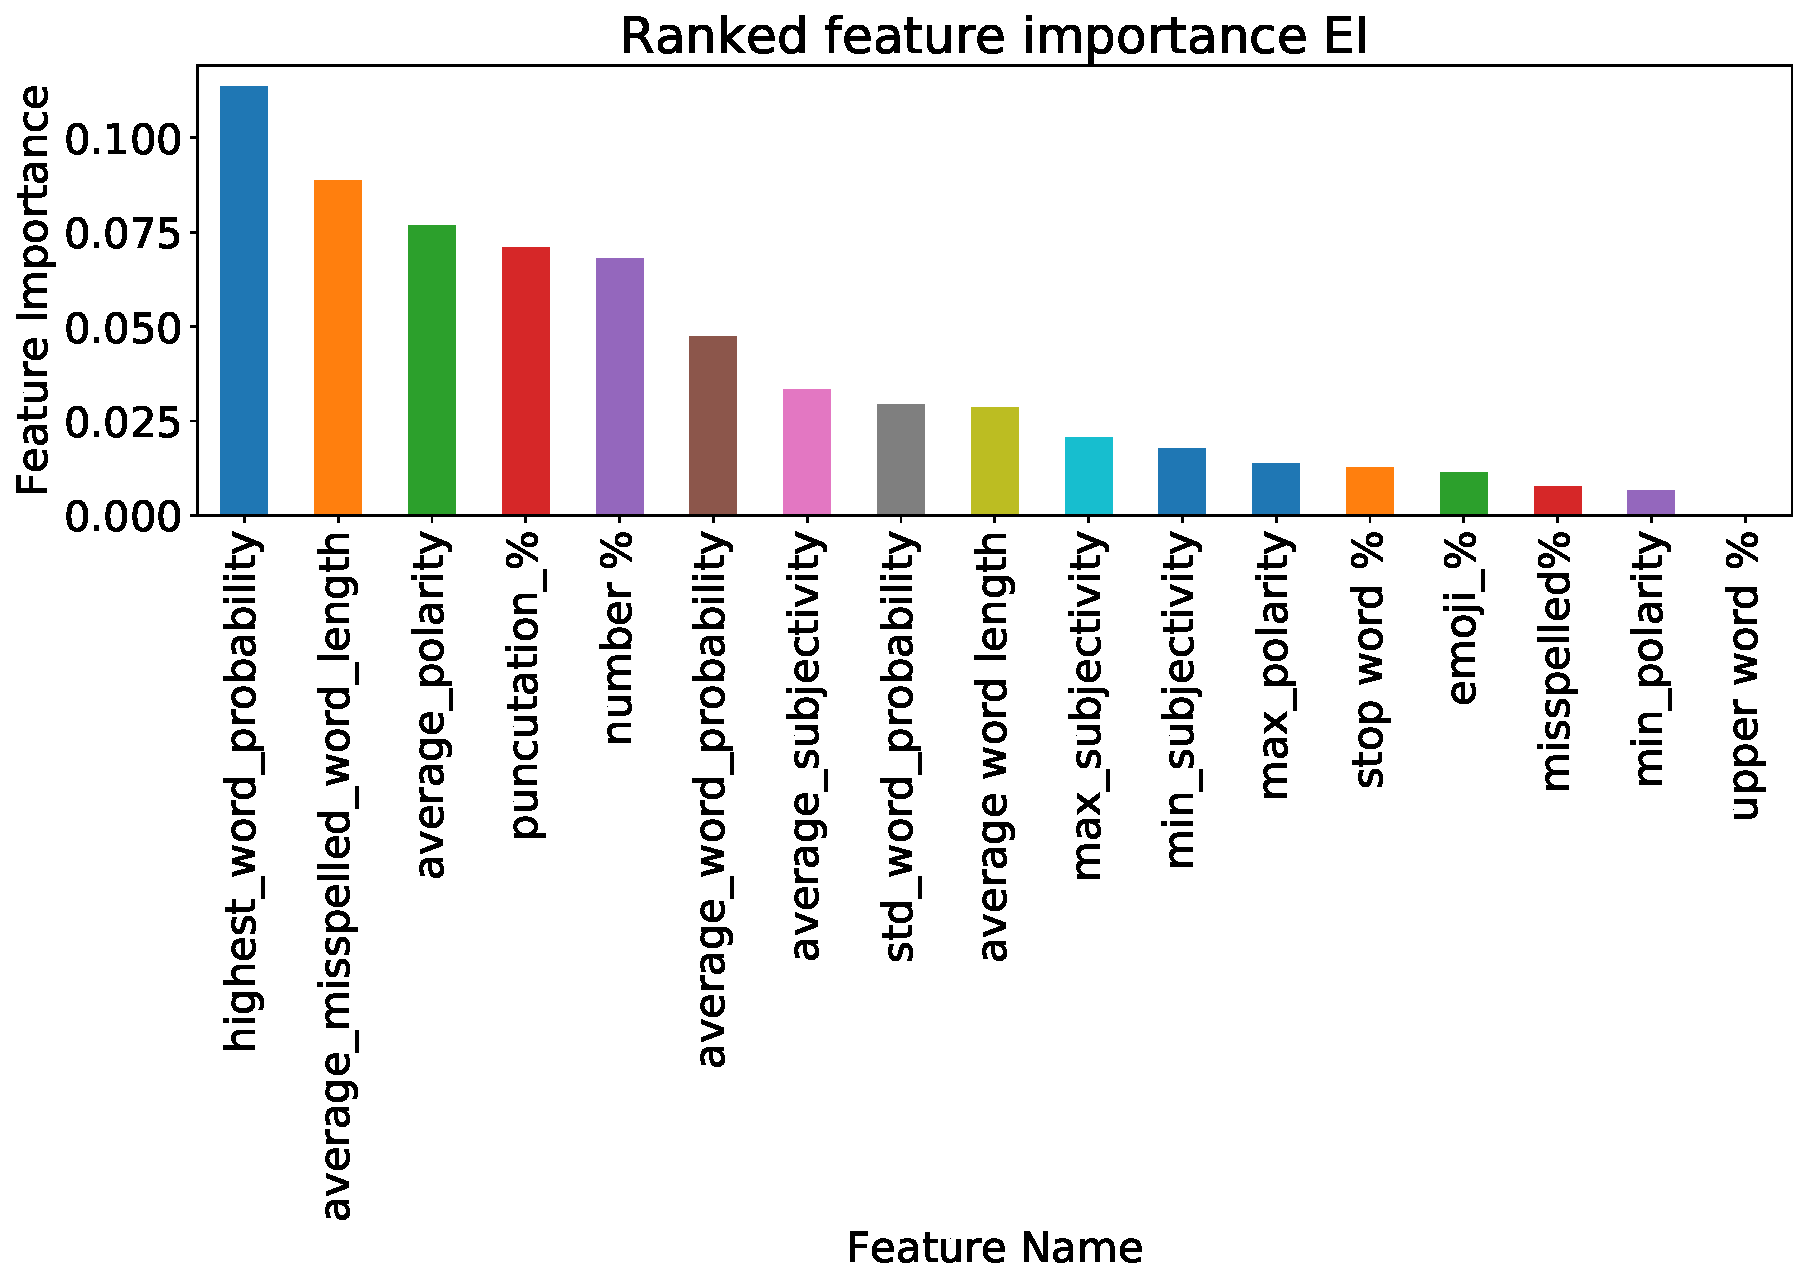
\includegraphics[width = 0.9\columnwidth]{EI.pdf} \\
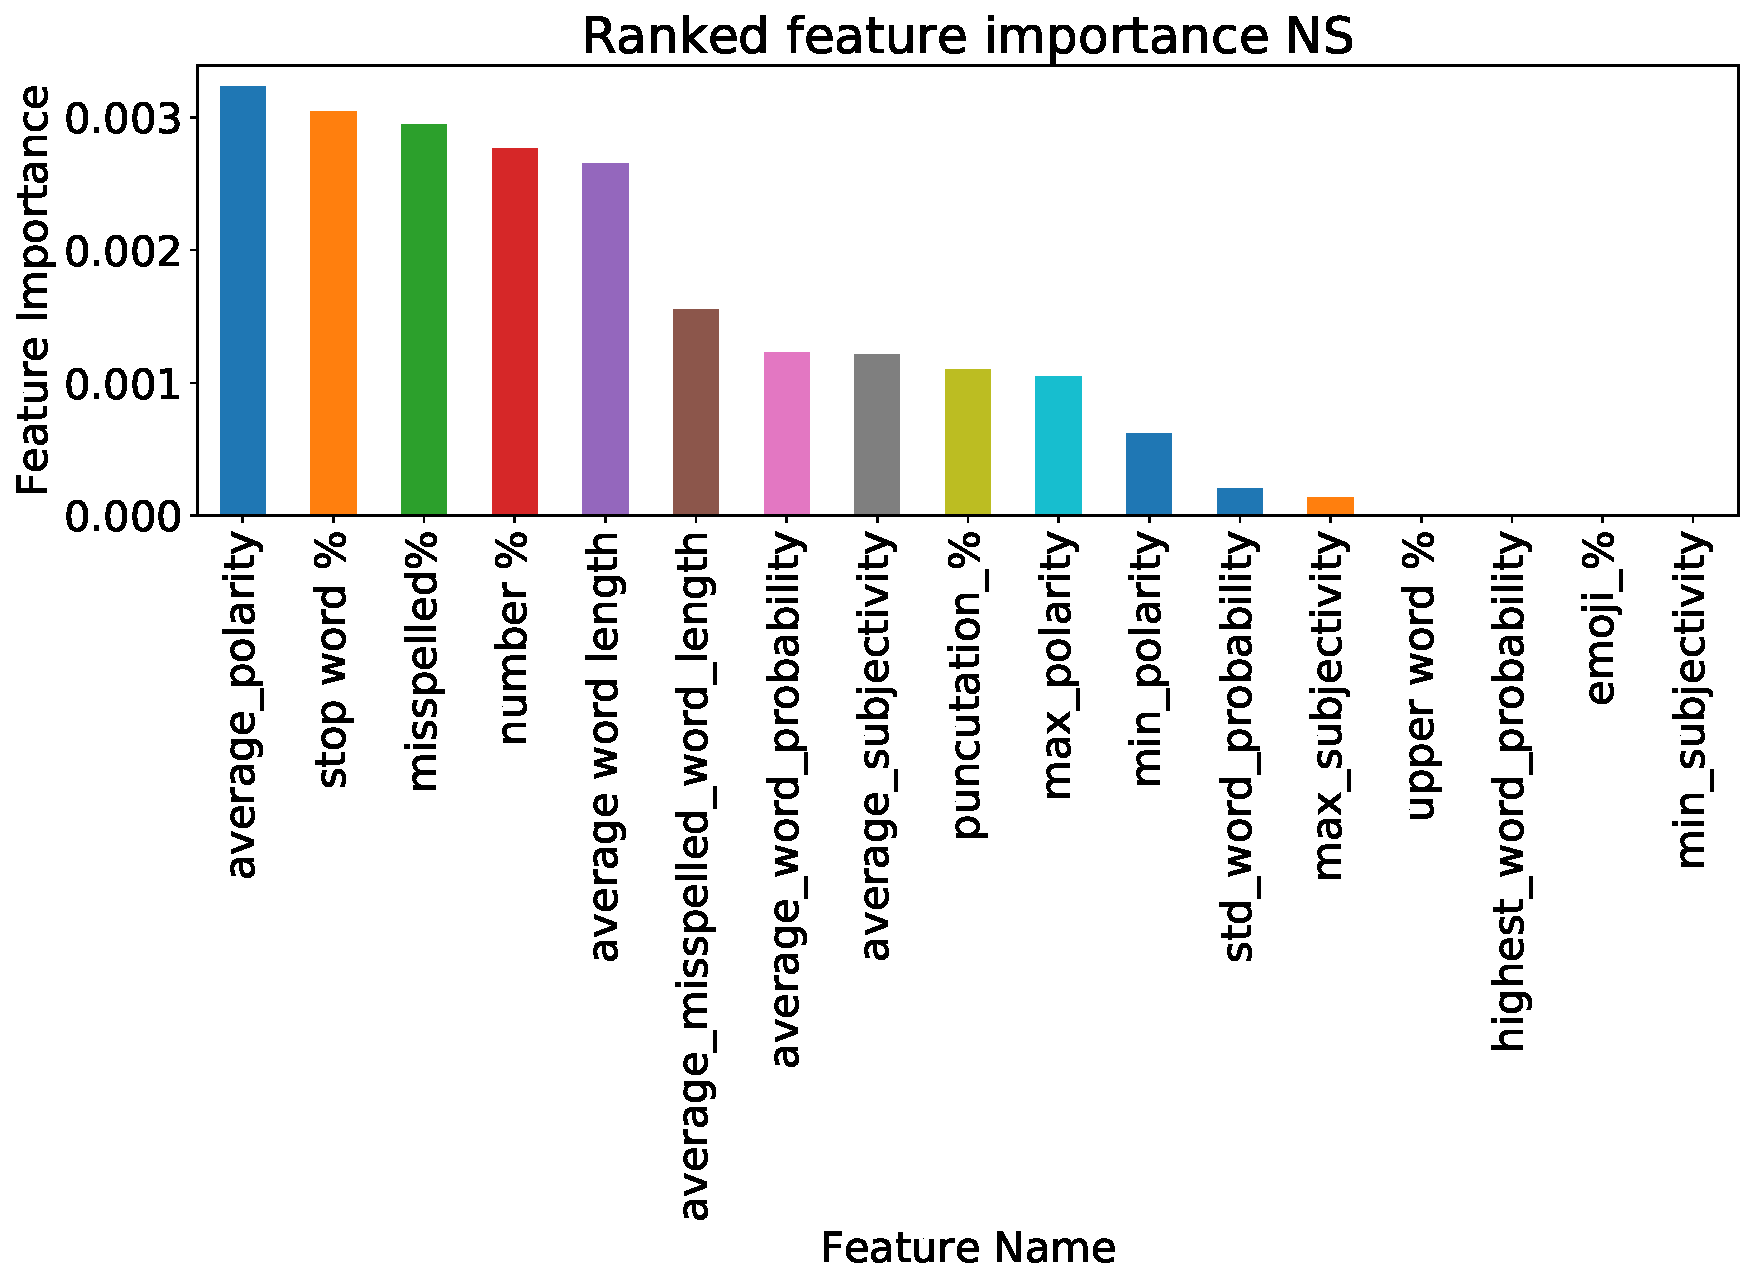
\includegraphics[width = 0.9\columnwidth]{NS.pdf} \\
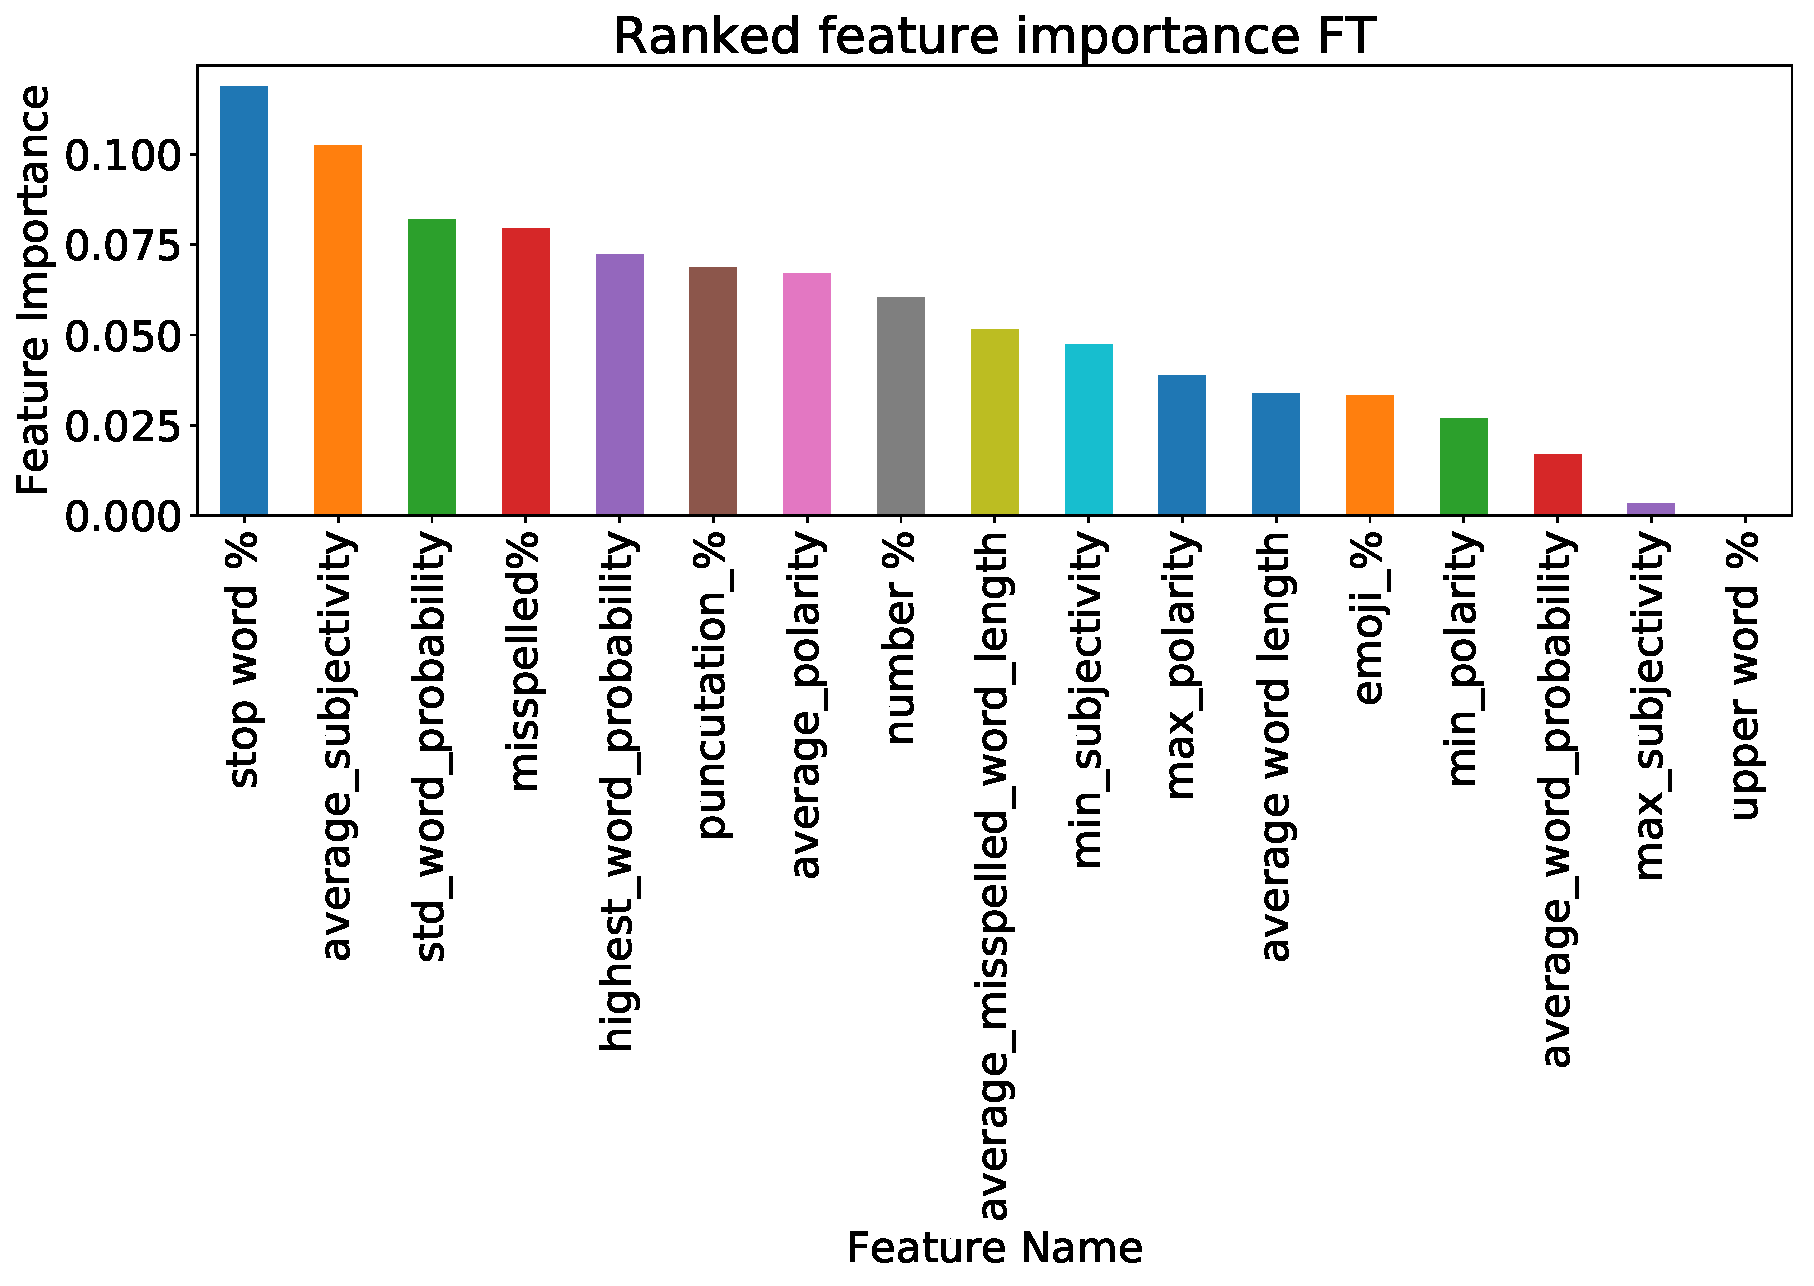
\includegraphics[width = 0.9\columnwidth]{FT.pdf} \\
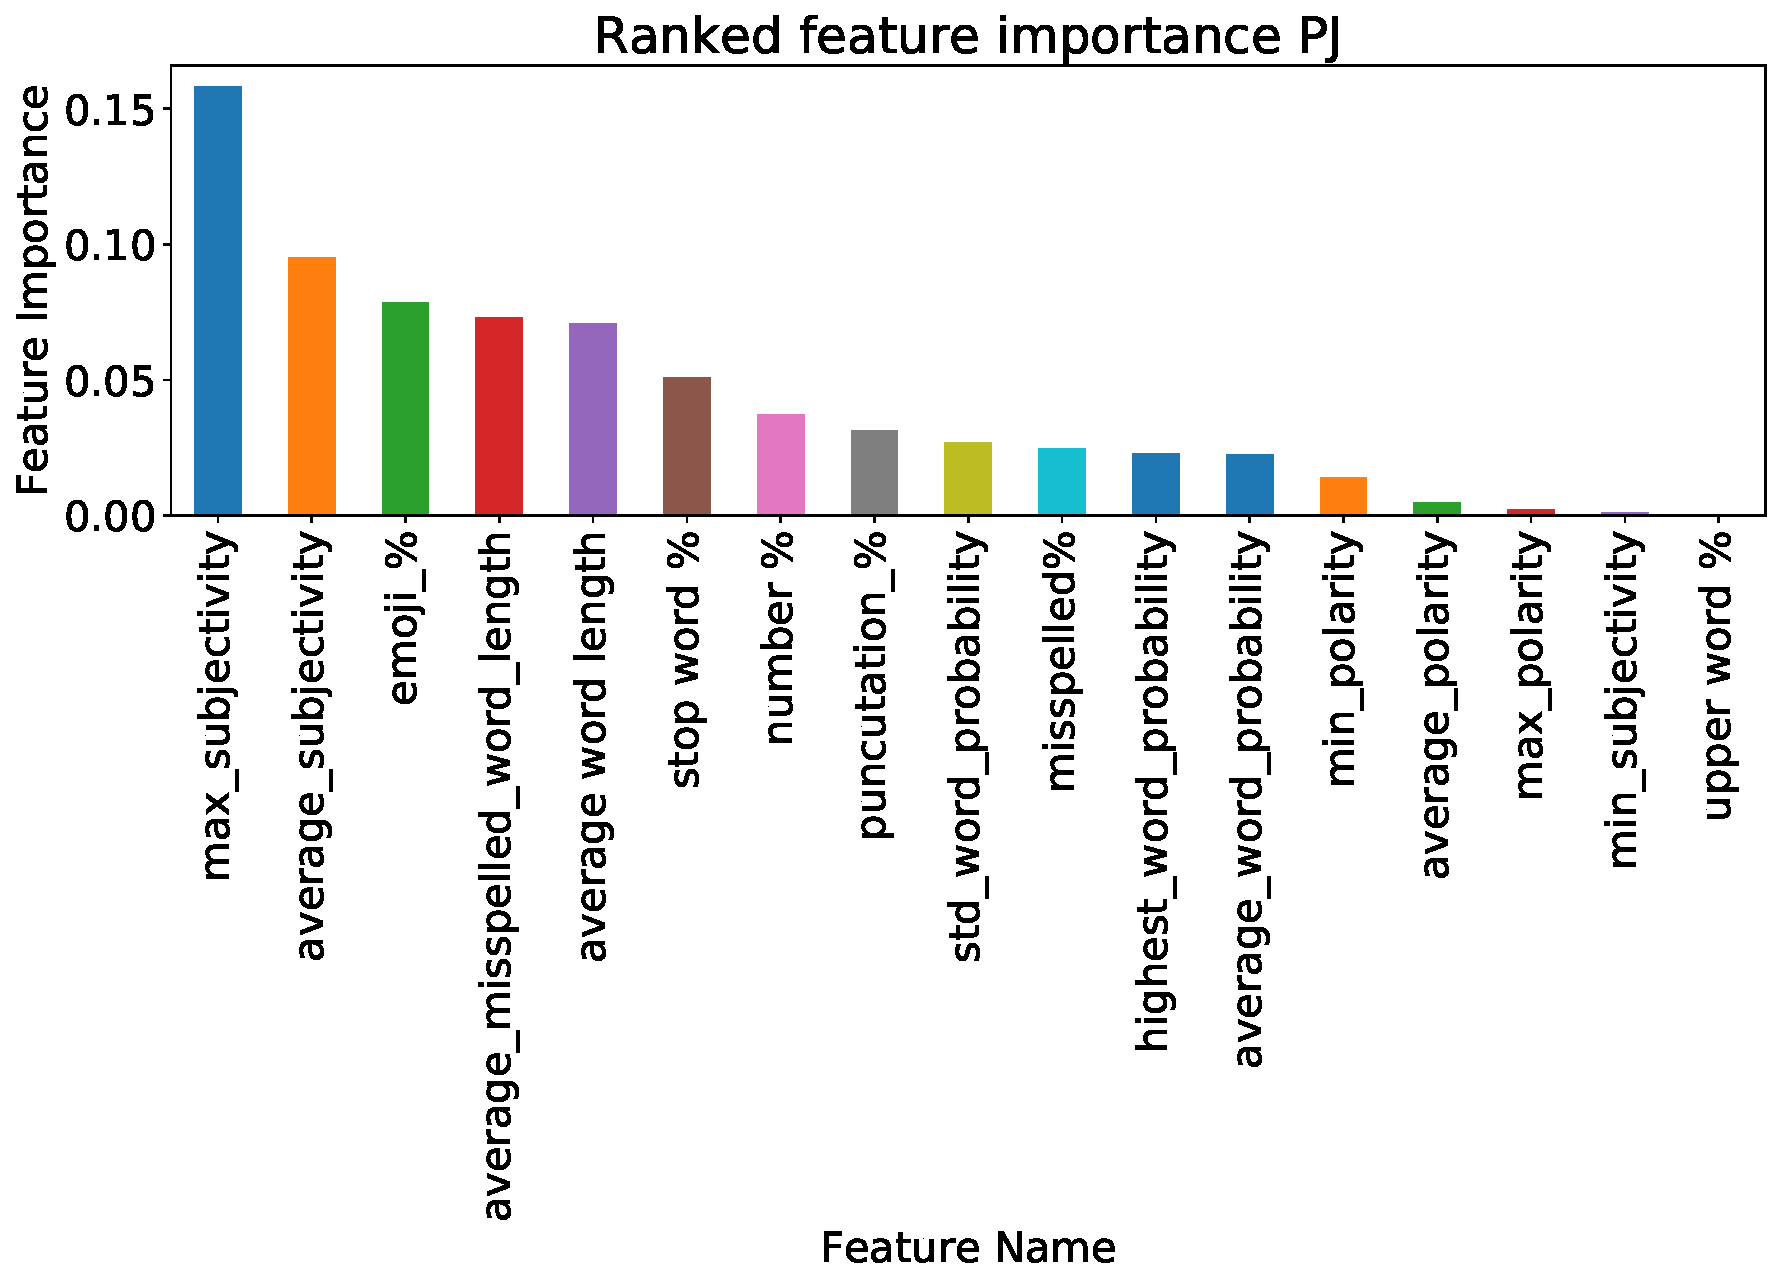
\includegraphics[width = 0.9\columnwidth]{PJ.pdf}
\end{tabular}
\caption{The ranking of engineered features in each of the predictive models. }
\label{feature_importance}
\end{figure}

\begin{table}[h!]
\centering
\begin{tabular}{ |p{2.5cm}|p{0.8cm}|p{0.8cm}|p{0.8cm}|p{0.8cm}|  }
 \hline
 \multicolumn{5}{|c|}{ML Models Results} \\
 \hline
ML Model&  E/I & F/T & N/S & P/J\\
 \hline
 Logistic Regression & 0.826 & 0.952 & 0.743 & 0.909\\
 SVM & 0.826 & 0.952 & 0.709 & 0.927\\
 Random Forest & 0.825 & 0.883 & 0.780 & 0.793\\
 Neural Network & 0.770 & 0.873 & 0.680 & 0.827\\
 \hline
\end{tabular}
\caption{The accuracy scores of the best predictive models using each of the machine learning approaches applied to each of unseen test sets for each of the letters that constitute a personality type according to Myres Briggs typology.}


\label{ModelResults}
\end{table}
\begin{figure}[h]
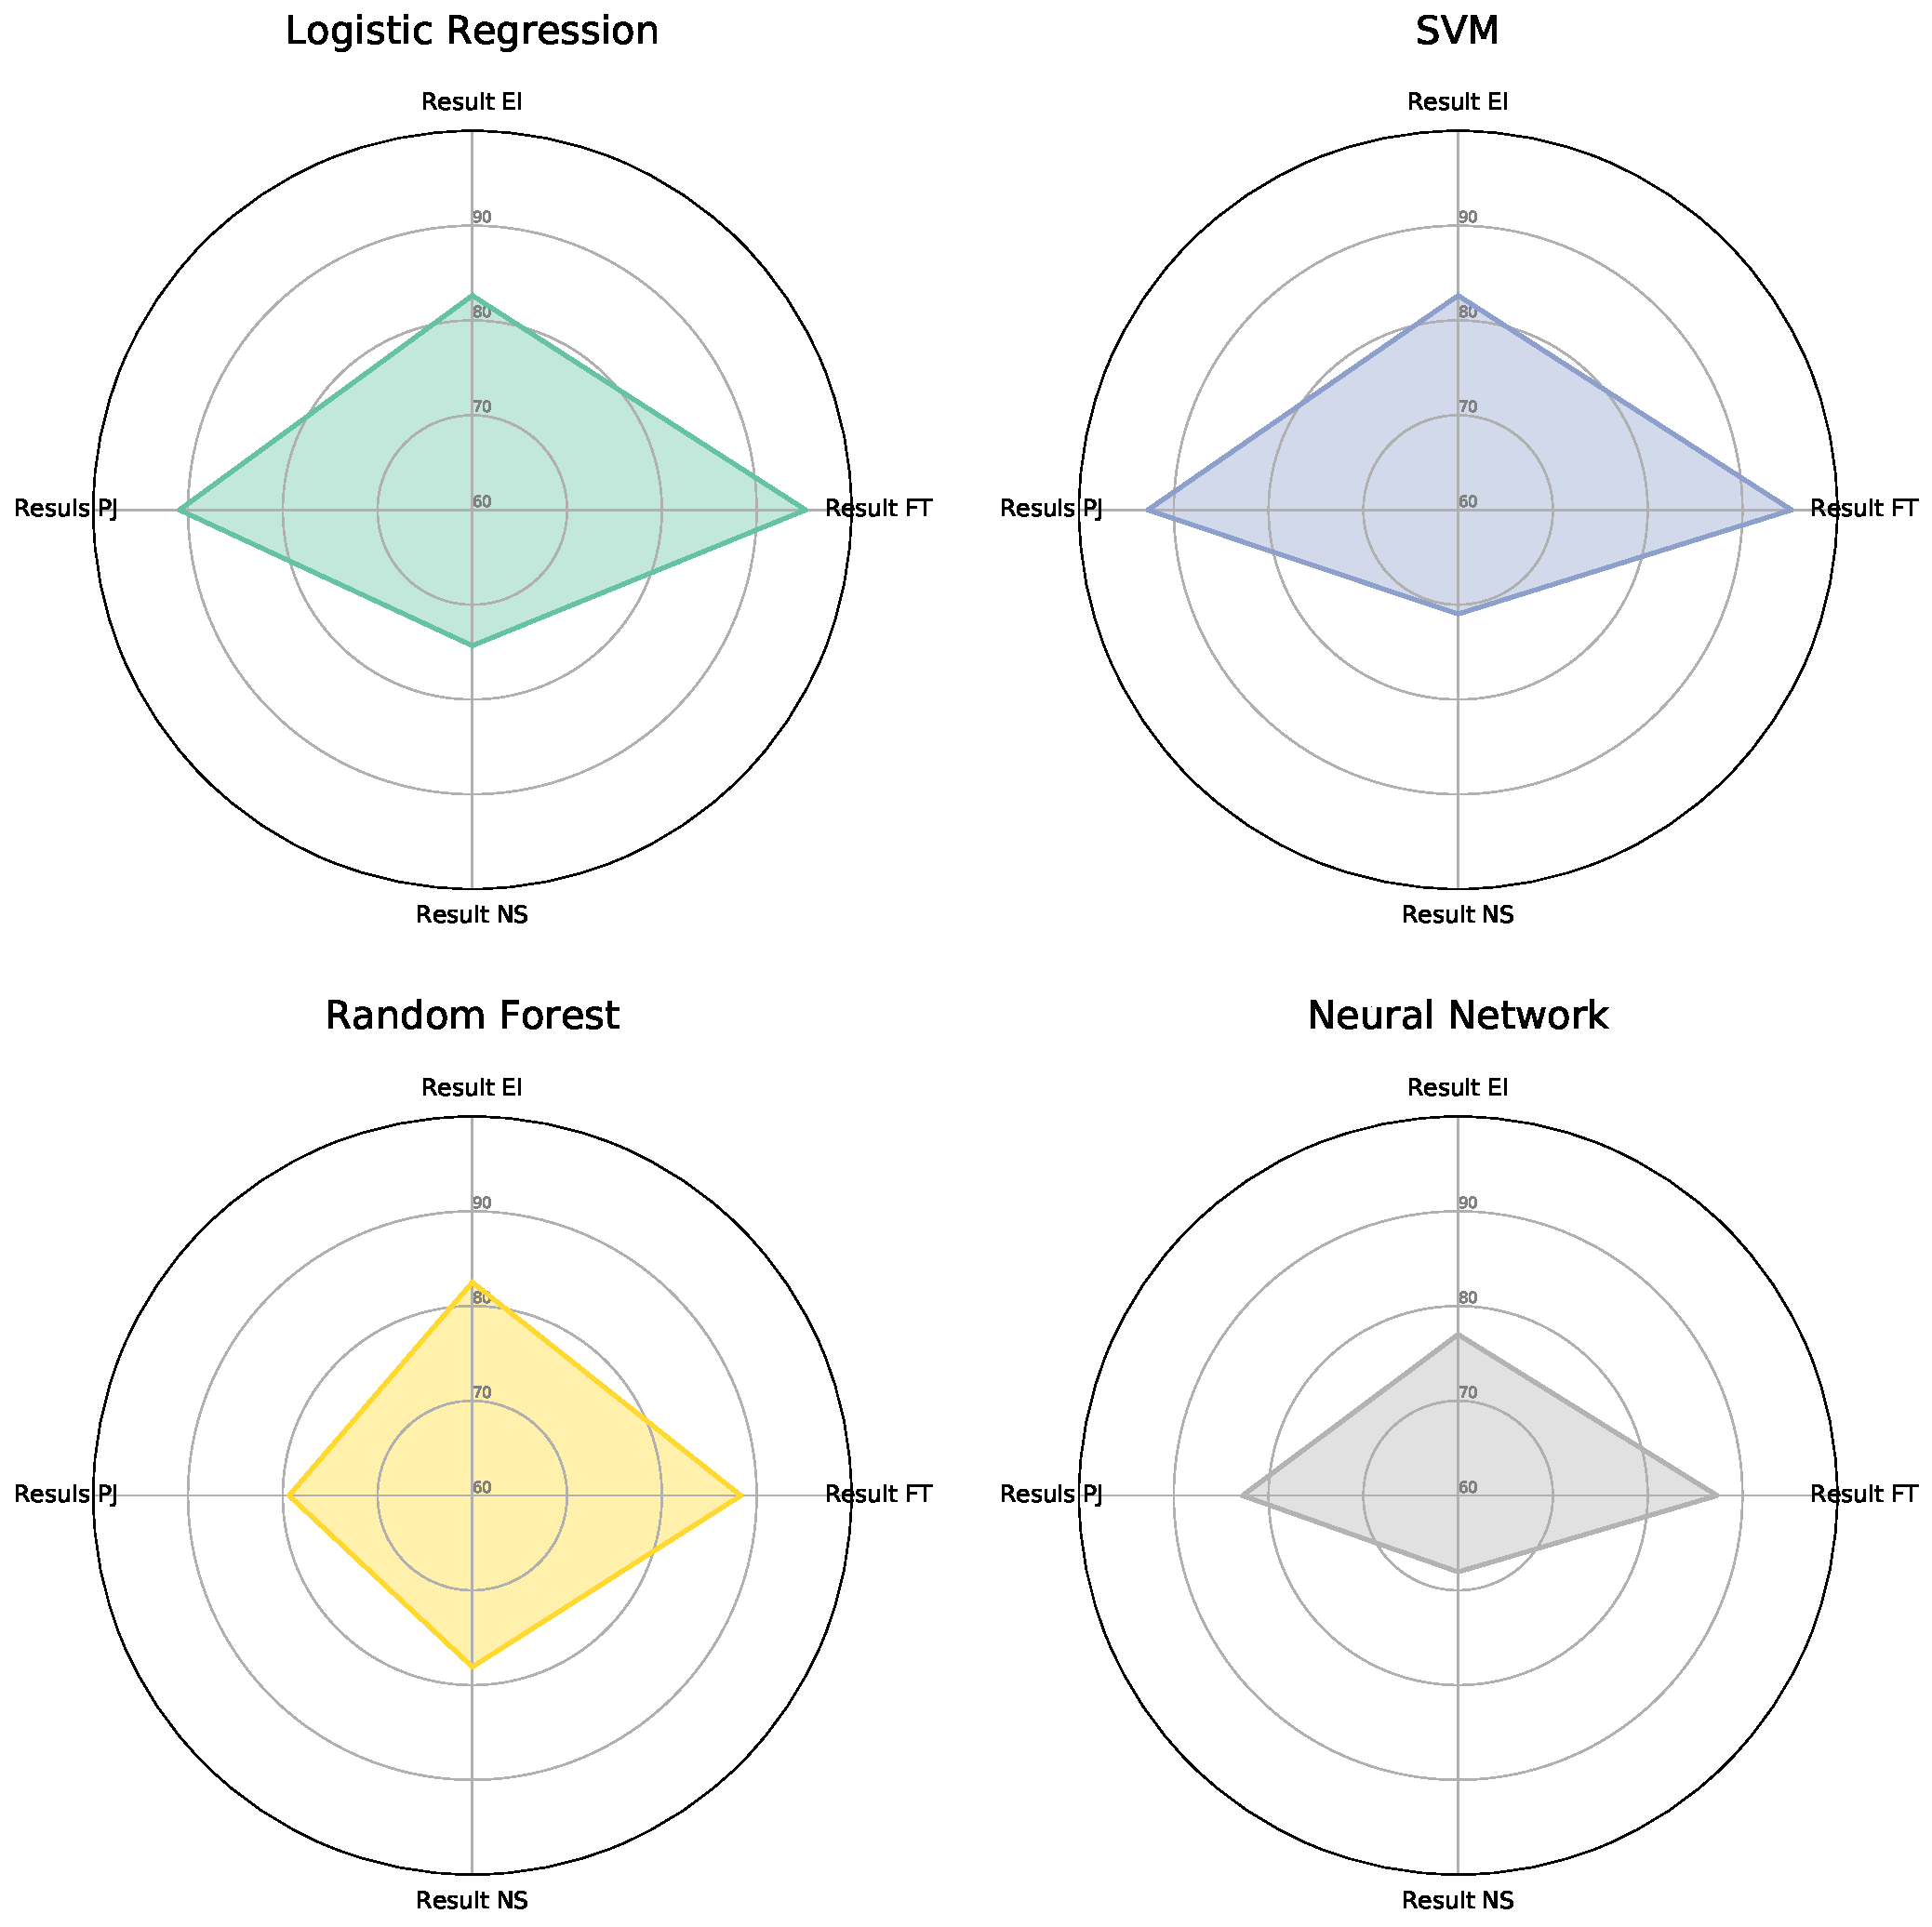
\includegraphics[width=0.9 \columnwidth]{results}
\caption{Here we shown the accuracy scores for each of the machine learning approaches in building predictive models for the 4 binary letter choices. }
\label{fig_ml_models_results}
\end{figure}


\section{Analysis}

After applying the best performing predictive models as selected by accuracy against the test set in the previous section to the Yelp dataset, we obtain a four letter personality for each of the reviewers. We present next some key findings.\\

Firstly, the distribution of personalities in Figure \ref{distribution_personalities}. In determining the validity of these results we look to research into the true distribution of personality types, although there are some samples collected for teachers and project managers \cite{cohen2013mbti, levy1972personality, furnham1993personality}, as far as we are aware, there are no meta studies of the general population. We instead look to the MBTI manual \cite{myers1998mbti}, which estimates the global distribution from multiple of sources and present the most frequent types in Table \ref{type_frequency}. Here we can see that whilst the E/I and N/S letters follow a distribution similar distribution of that found in the general population, that there is some discrepancy between the latter two letters F and J. It is difficult to know for certain whether the true distribution of personality letters in the Yelp dataset are closer to that of our results and of that found in \cite{boyle1995myers} but it is a point of notice which warrants further investigation. \\


\begin{center}
\begin{table}
\begin{tabular}{| c | c | c | c |}
\hline 
Letter & Yelp distribution & MBTI distribution  & Difference \\
\hline
I & 48.5\% & 42\% & +6.5\% \\ 
N & 25.8\% & 26.6\% & -0.8\% \\
F & 92\% & 59\% & +37\% \\
J & 15.3 & 54.5\% & -39\% \\
\hline



\end{tabular}
\caption{A table comparing the distribution of personality letters in the Yelp dataset as determined by the predictive model and that found in the MBTI manual \cite{myers1998mbti}} 
\label{type_frequency}
\end{table}
\end{center}


\begin{center}
\begin{figure}
\begin{tabular}{ c c }
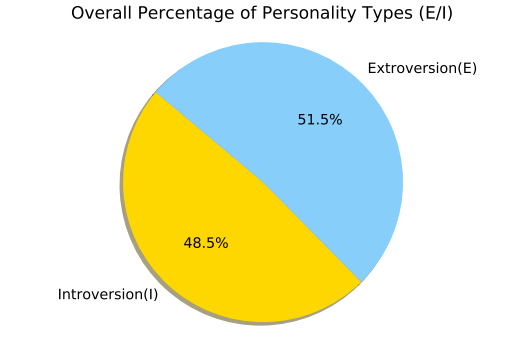
\includegraphics[width = 0.4\columnwidth]{E_I_Dist} & 
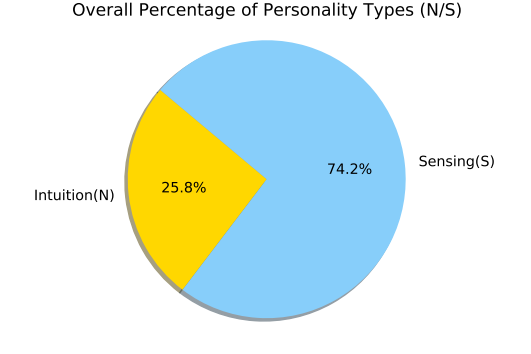
\includegraphics[width = 0.4\columnwidth]{N_S_Dist} \\
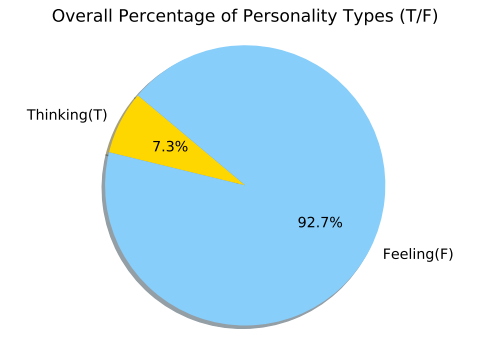
\includegraphics[width = 0.4\columnwidth]{T_F_Dist} & 
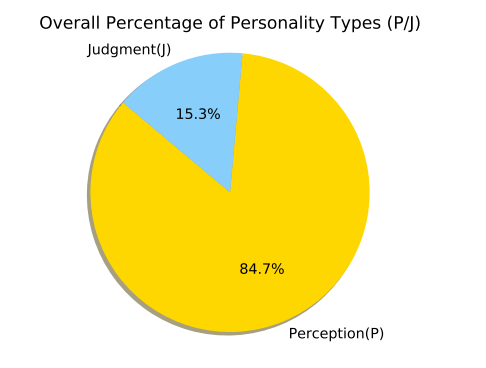
\includegraphics[width = 0.4\columnwidth]{P_J_Dist} 
\end{tabular}
\caption{The distribution of personalities found after applying the predictive model to the Yelp dataset.}
\label{distribution_personalities}
\end{figure}
\end{center}


Interesting, we see a small but notable difference in the distribution of ratings given by each of the letter types, which we give in Figure \ref{ratings}. Whilst, this difference is small, we do notice a larger variance of ratings by letter depending on which business the reviews are for. It is this, the difference in ratings allocated by personality by business which motivates the application which we next discuss.  \\

\begin{center}
\begin{figure}
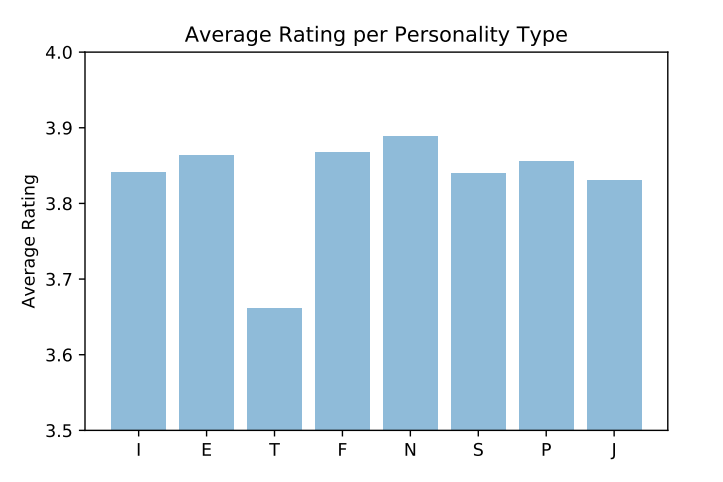
\includegraphics[width = 0.9\columnwidth]{ratings.png}
\caption{The average ratings given in the Yelp dataset  by personality type}
\label{ratings}
\end{figure}
\end{center}


\section{Application}

We next present a personality model application. For demonstrative purposes, we take the results of the Yelp data with appended personalities after applying the machine learning models and produce an application to inform Yelp using business. \\

\begin{center}
\begin{figure}
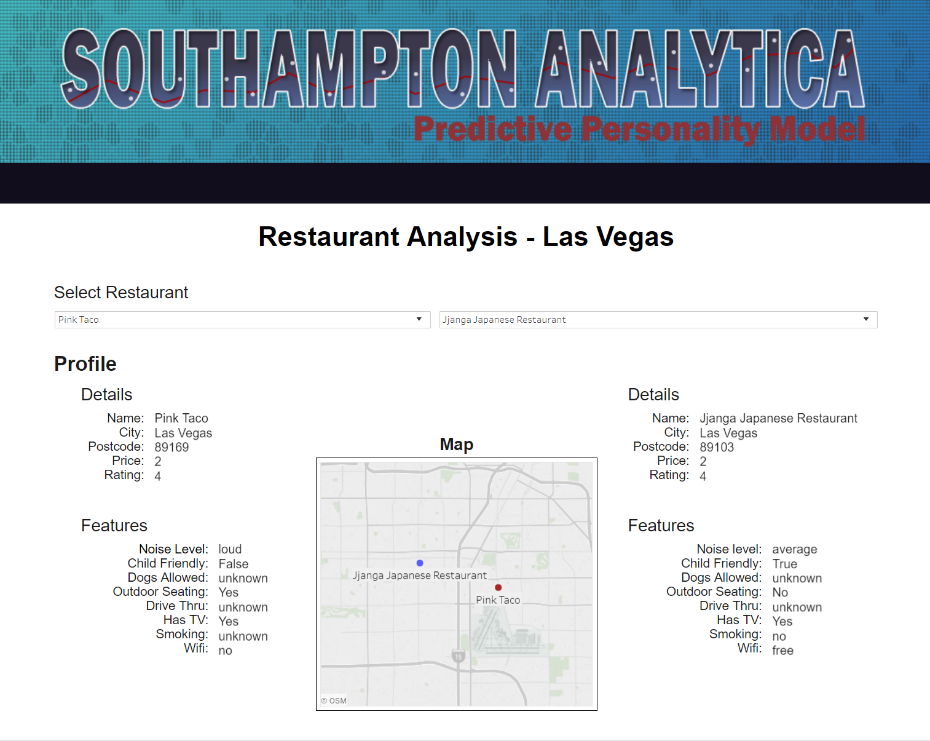
\includegraphics[width = 0.9 \columnwidth]{top_app}
\caption{The main application view, where businesses can be selected and mapped based on locational data}
\label{top_app}
\end{figure}
\end{center}

\begin{center}
\begin{figure}
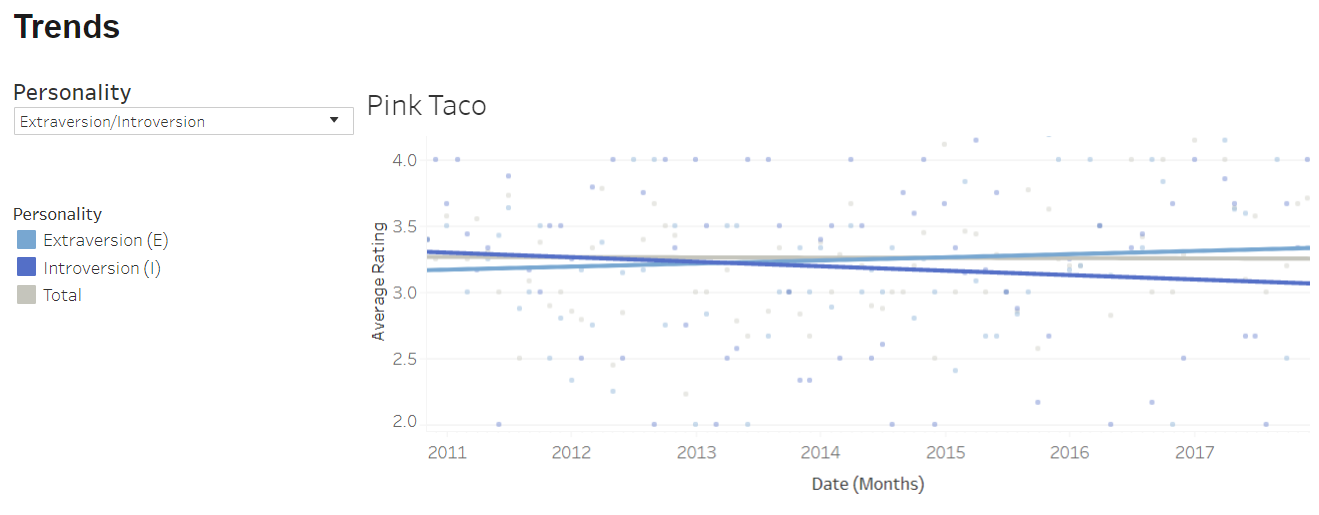
\includegraphics[width = 0.9 \columnwidth]{bottom_app}
\caption{The trends chart in the application. In this example we observe that the personality average rating switches in 2013, despite the total average rating staying relatively static. This infers that the business has appealed more to extroverted customers in recent years. }
\label{bottom_app}

\end{figure}
\end{center}



The application is intended for broad analysis, allowing for two businesses in the processed dataset to be compared against each other. It displays relevant metrics already present in the Yelp dataset, such as price ranges and location (shown in Figure \ref{top_app}) and provides a word cloud, generated from the 50 most frequent terms (after eliminating stop words) giving an overview of the language being used.  \\


Additionally it allows the business to explore how ratings are distributed by personality types. We achieve this by graphing the distribution of user ratings for each of the applicable personality types as well through trend charts, which reflect the average user ratings overtime by personality (presented in Figure \ref{bottom_app}).  \\

This added functionality enables the tool to be used by a business to evaluate and understand trends in ratings given by reviews of varying personalities.   \\

We further motivate the application with the following: If a business wants to improve its customer satisfaction, as captured in rating response, should it concentrate on moderate service users that are of a personality type that it currently enjoys success with? Or should it look to similar businesses which are doing well with customers of a personality type that it is not, and try to understand and emulate its success? \\

Our analysis and application allows for such questions to be asked where before they could not. Further iterations will look to build upon these features with the intention to gain feedback from potential users of the business of any improvements. 

\section{Discussion}

We start with some limitations with our works. Firstly the use of MBTI as a way of categorising personality has some notable limitations \cite{boyle1995myers} and another set of personality determinants, such as the Big Five \cite{gosling2003very} could very well be more informative and considered for future models. \\

We also note that building predictive models on one source of data and using this model to make predictions on another source of data can prove inaccurate since the underlying distributions, and therefore patterns used in making the predictions, could be very different leading to inaccuracies. This could account for the variation in observed distributions of personalities in the Yelp data and of that found in the literature. \\

That said, our models have strong predictive accuracy which are able to, given some strong assumptions about the universal nature of language structure of persons of particular personality types, be applied to other similar text datasets to create a prototype application of commercial use. \\

We envision that, with further work improving the models ability to be applied to multiple sources, this application could be used in understanding the distribution of personalities in a wider set of contexts. \\


\section{Conclusion}

We have explored an application of machine learning in determining the personality of Yelp business reviews. Using these predictions we then demonstrated the potential utility through the building of a review analytics application which provides a granular understanding of the role of personalities in the distribution of review ratings. Our results show that the distribution of ratings vary across different personality types and that these change over time. This could in the future allow businesses to monitor and react to user base responses to marketing strategies at a personality trait level and give valuable insight into the nature of reviewers.

\section{Application Link}

Avaliable at: https://jakhall.github.io/southampton-analytica/

\\
Email login: sa.guest@email.com \\
Password: guest.19 

\bibliography{yelp_review_personailities.bib}
\bibliographystyle{ieeetr}


\end{document}
